% IK Tau
\begin{figure*}
\centering
  \begin{subfigure}{\hsize}
    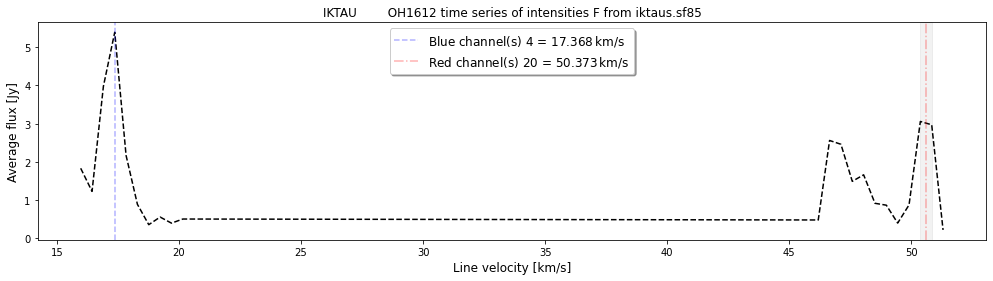
\includegraphics[width=0.95\hsize]{images/IKTau_avg_spectrum.png}
    \caption{\label{fig:iktauspectrum}Spectral profile show double narrow red peaks with no noticeable emission in between the blue peak and the red peaks. For flattened peak structures, such as for the red peaks, an average of the channels over that flat peak was used, rather than a single channel.}
  \end{subfigure}%
  \\
  \begin{subfigure}{\hsize}
    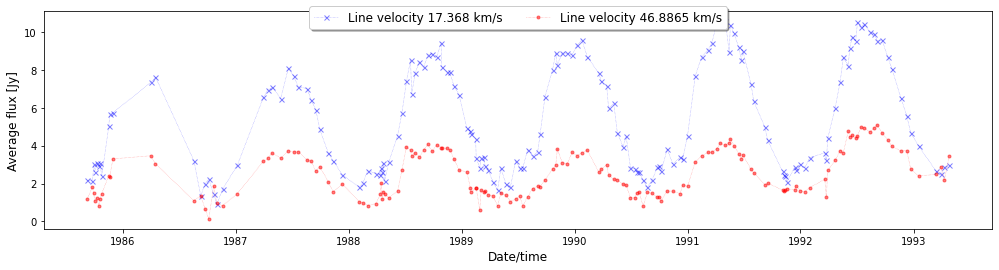
\includegraphics[width=0.95\hsize]{images/IKTau_ts_blue4_red12.png}
    \caption{\label{fig:iktautimeseries0}Time series of red peak show significantly weaker signal than blue peak. Both blue and red time series show similar behaviour over the monitoring period with a slow linear increase in baseline (most noticeable toward the end) and consistent amplitude over time.}
  \end{subfigure}%
  \\
  \begin{subfigure}{\hsize}
    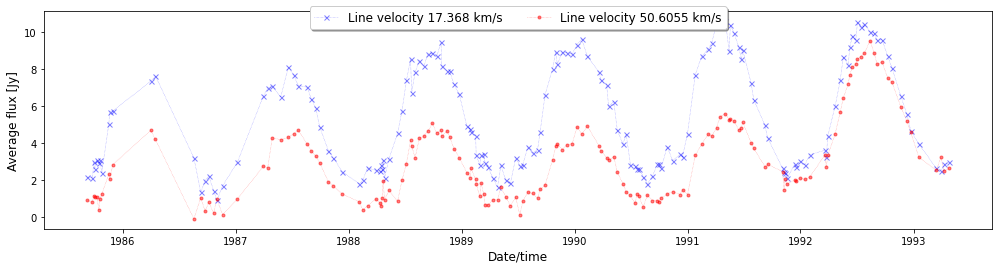
\includegraphics[width=0.95\hsize]{images/IKTau_ts_blue4_red20.png}
    \caption{\label{fig:iktautimeseries1}The time series data for this peak show significant changes during the last monitoring cycle with not only a strong increase in baseline, but also a significant increase in strength with the amplitude of the last cycle comparable to the amplitude of the stronger blue line.}
  \end{subfigure}%
\caption{\label{fig:iktau}The 1612 MHz OH spectrum of IK Tau at maximum and minimum light.}
\end{figure*}

\begin{figure*}
\centering
  \begin{subfigure}{0.33\hsize}
    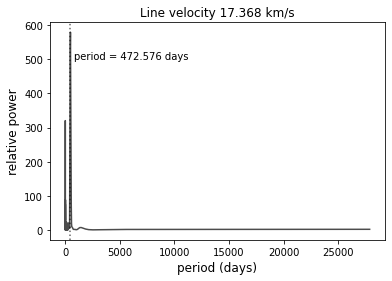
\includegraphics[width=0.99\hsize]{images/IKTau_blue_17.368_periodogram.png}
  \end{subfigure}%
  \hfill
  \begin{subfigure}{0.33\hsize}
     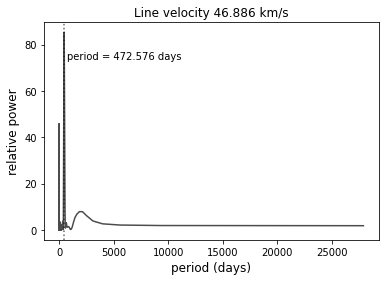
\includegraphics[width=0.99\hsize]{images/IKTau_red_46.886_periodogram.png}
  \end{subfigure}%
  \hfill
  \begin{subfigure}{0.33\hsize}
    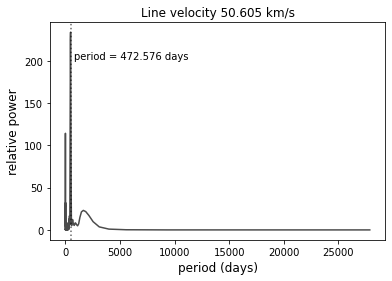
\includegraphics[width=0.99\hsize]{images/IKTau_red_50.605_periodogram.png}
  \end{subfigure}%
\caption{\label{fig:iktauperiod}Lomb-Scargle periodogram calculations for IK Tau blue and red channel time series data give average period of 472.576 days.}
\end{figure*}


% VMic
\begin{figure*}
\centering
  \begin{subfigure}{\hsize}
    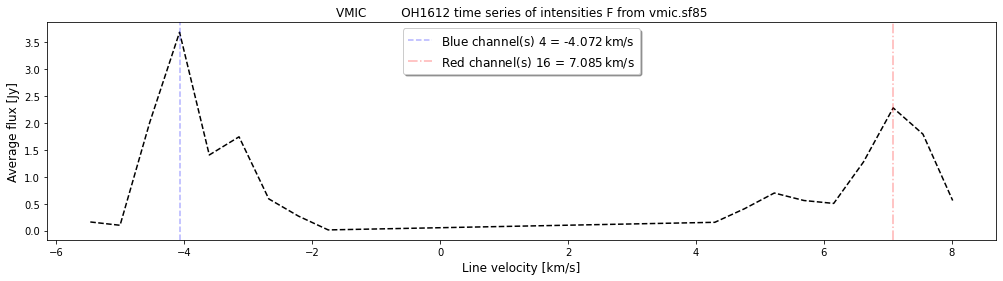
\includegraphics[width=0.95\hsize]{images/VMic_avg_spectrum.png}
    \caption{\label{fig:vmicspectrum}Identification of the the blue and red channels are not well defined narrow peaks, so simple maximum value evaluation was used for channel selection.}
  \end{subfigure}%
  \\
  \begin{subfigure}{\hsize}
    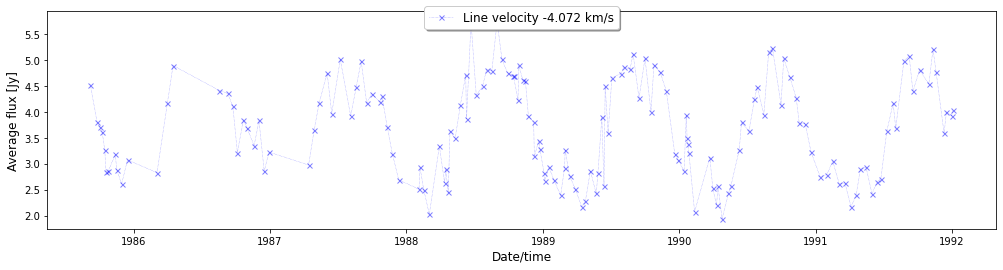
\includegraphics[width=0.95\hsize]{images/VMic_ts_blue4.png}
    \caption{\label{fig:vmictimeseries}Since V Mic is such a weak source, it is difficult to distinguish the time series data for the blue (-4.072 km/s) and red (7.085 km/s) channels if plotted in overlay. For this reason only the the time series for the stronger blue channel is displayed.}
  \end{subfigure}%
\caption{\label{fig:vmic}The 1612 MHz OH spectrum of VMic at maximum and minimum light.}
\end{figure*}

\begin{figure*}
\centering
  \begin{subfigure}{0.5\hsize}
    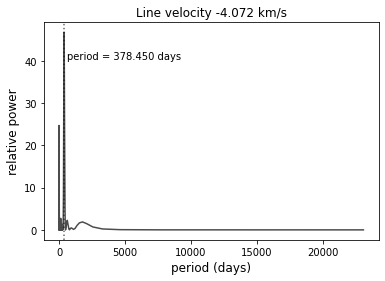
\includegraphics[width=0.99\hsize]{images/VMic_blue_-4.072_periodogram.png}
  \end{subfigure}%
  \hfill
  \begin{subfigure}{0.5\hsize}
    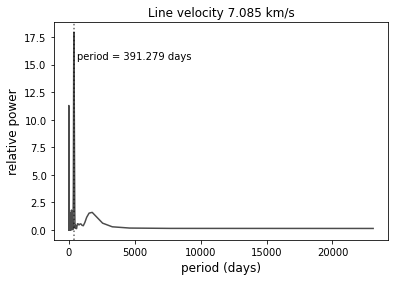
\includegraphics[width=0.99\hsize]{images/VMic_red_7.085_periodogram.png}
  \end{subfigure}%
\caption{\label{fig:vmicperiod}Lomb-Scargle periodogram calculations for V Mic blue and red channel time series data give differing period for the blue and red channels. This difference is expected since the source is weak, but the average period of 384.86 days gives a reasonably good fit to the data and agrees well with the stellar period.}
\end{figure*}

\begin{figure*}
\centering
  \begin{subfigure}{\hsize}
%    \includegraphics[width=0.95\hsize]{images/}
    \caption{Spectral profile show narrow peaks with no noticeable emission in between.}
    \label{fig:wxpscspectrum}
  \end{subfigure}%
  \\
  \begin{subfigure}{\hsize}
%    \includegraphics[width=0.95\hsize]{images/}
    \caption{Light curves of brightest peaks are averaged power of neighbouring blue- and red-shifted peaks.}
    \label{fig:wxpsctimeseries}
  \end{subfigure}%
\caption{\label{fig:wxpsc}The 1612 MHz OH spectrum and light curve of WX Psc at maximum and minimum light.}
\end{figure*}


\begin{figure*}
\centering
  \begin{subfigure}{\hsize}
    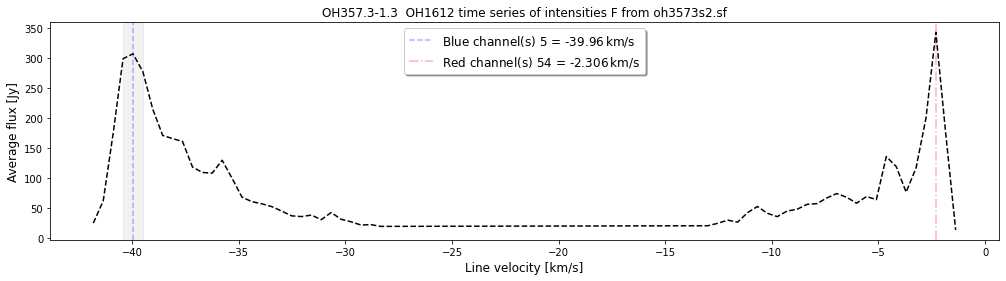
\includegraphics[width=0.95\hsize]{images/OH357_avg_spectrum.png}
    \caption{\label{fig:oh357spectrum}Spectral profile showing the canonical `U' shape of a spherical dust shell around OH/IR stars. The spectrum show clear blue and red peaks, with the blue peak taken to be the average of the 3 channels at maximum.}
  \end{subfigure}%
  \\
  \begin{subfigure}{\hsize}
    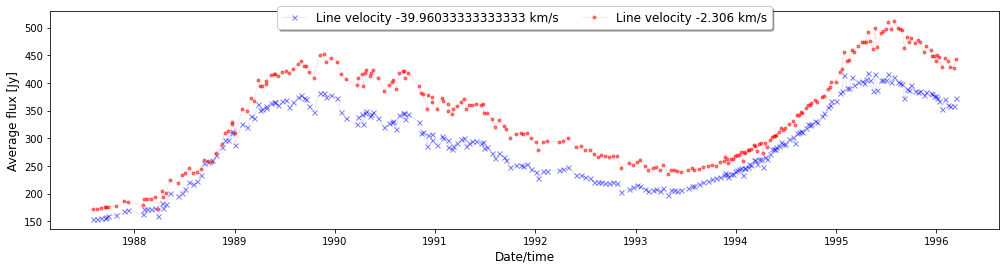
\includegraphics[width=0.95\hsize]{images/OH357_ts_blue5_red54.png}
    \caption{\label{fig:oh357timeseries}Time series of brightest blue- and red-shifted peaks show single period over 6 years. The second peak of the red channel sow a mark increase in amplitude and asymmetry in shape. Visually there seem to be some delay between the 2 signals.}    
  \end{subfigure}%
\caption{\label{fig:oh357}The 1612 MHz OH spectrum and light curve of OH357.1--1.3 at maximum and minimum light.}
\end{figure*}

\begin{figure*}
\centering
  \begin{subfigure}{\hsize}
    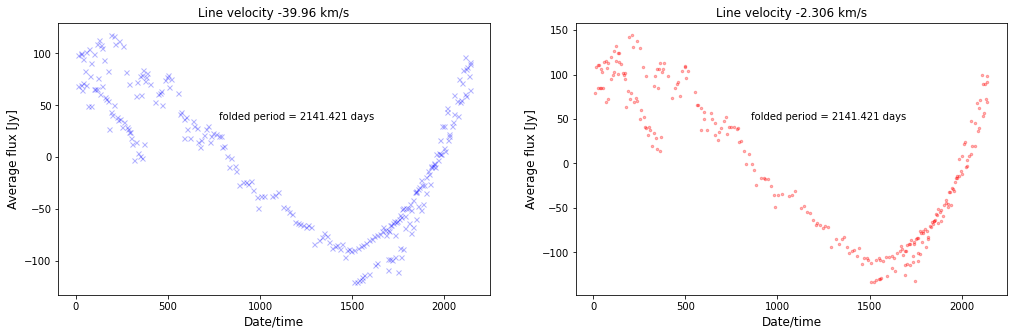
\includegraphics[width=0.99\hsize]{images/OH357_ts_blue5_red54_detrended_folded.png}
  \end{subfigure}%
\caption{\label{fig:oh357period}Folded time series for manually established best fit period of 2141.421 days for both blue and red channels.}
\end{figure*}


\begin{figure*}
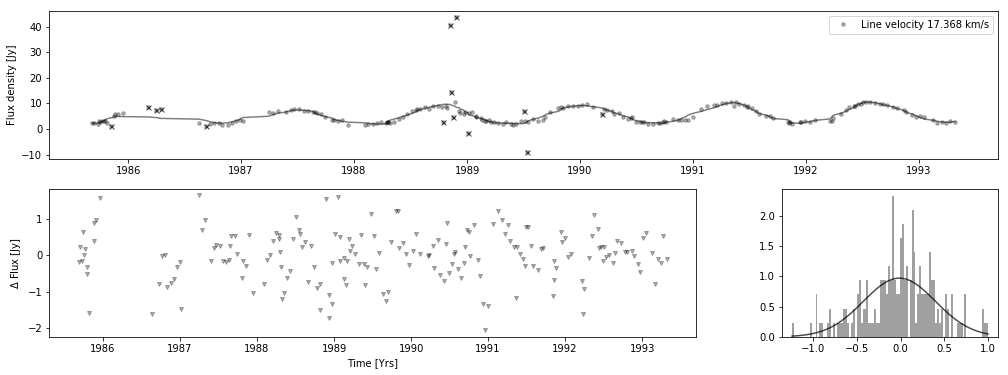
\includegraphics[width=\hsize, clip,angle=0]{images/iktausRAW_blue_channels_cleaned.png}
\caption{\label{fig:iktaublueclean}The dots in the top graph show the cleaned time series data for IK Tau blue channel. While the crosses indicates the discarded outliers. To evaluate how well the smoothed curve fit the data the residual is shown as triangles in the lower left plot. The histogram of the residual, lower right plot, is used for visual evaluation with the process continued until this distribution indicates a reasonable noise like character to the residual.}
\end{figure*}
